\documentclass{beamer}

\usecolortheme[light]{solarized}

\beamertemplatenavigationsymbolsempty

\usepackage{hyperref}

\usepackage{booktabs}
\usepackage{graphicx}
\usepackage{minted}
\usepackage{moresize}
\usepackage{standalone}
\usepackage{tcolorbox}
\usepackage{tikz}
\usepackage[normalem]{ulem}
\usepackage{xpatch}
\usepackage{amsmath}

\xpatchcmd{\sout}
  {\bgroup}
    {\bgroup\def\ULthickness{2pt}}
      {}{}

\usetikzlibrary{calc, patterns}

\definecolor{twitter}{RGB}{64, 153, 255}
\definecolor{github}{RGB}{211, 211, 211}

\newcommand{\assetsfolder}{./assets}
\newcommand{\researchfolder}{$HOME/rsc/axelrod-moran}
\newcommand{\mlresearchfolder}{$HOME/rsc/ml-paper}

\begin{document}

    \begin{frame}
        \begin{center}
            \Large
               Vince: \href{https://twitter.com/drvinceknight}{@drvinceknight}\\

               \href{https://arxiv.org/abs/1707.06920}{arxiv.org/abs/1707.06920}
               \vfill
               \begin{columns}
                   \begin{column}{.3\textwidth}
                       \begin{center}
                       
\includegraphics[height=3cm]{\assetsfolder/CUident_CMYK.eps}
                       \end{center}
                   \end{column}
                   \begin{column}{.3\textwidth}
                       \begin{center}
                       
\includegraphics[height=3cm]{\assetsfolder/ssi-logo.png}
                       \end{center}
                   \end{column}
                   \begin{column}{.3\textwidth}
                       \begin{center}
                       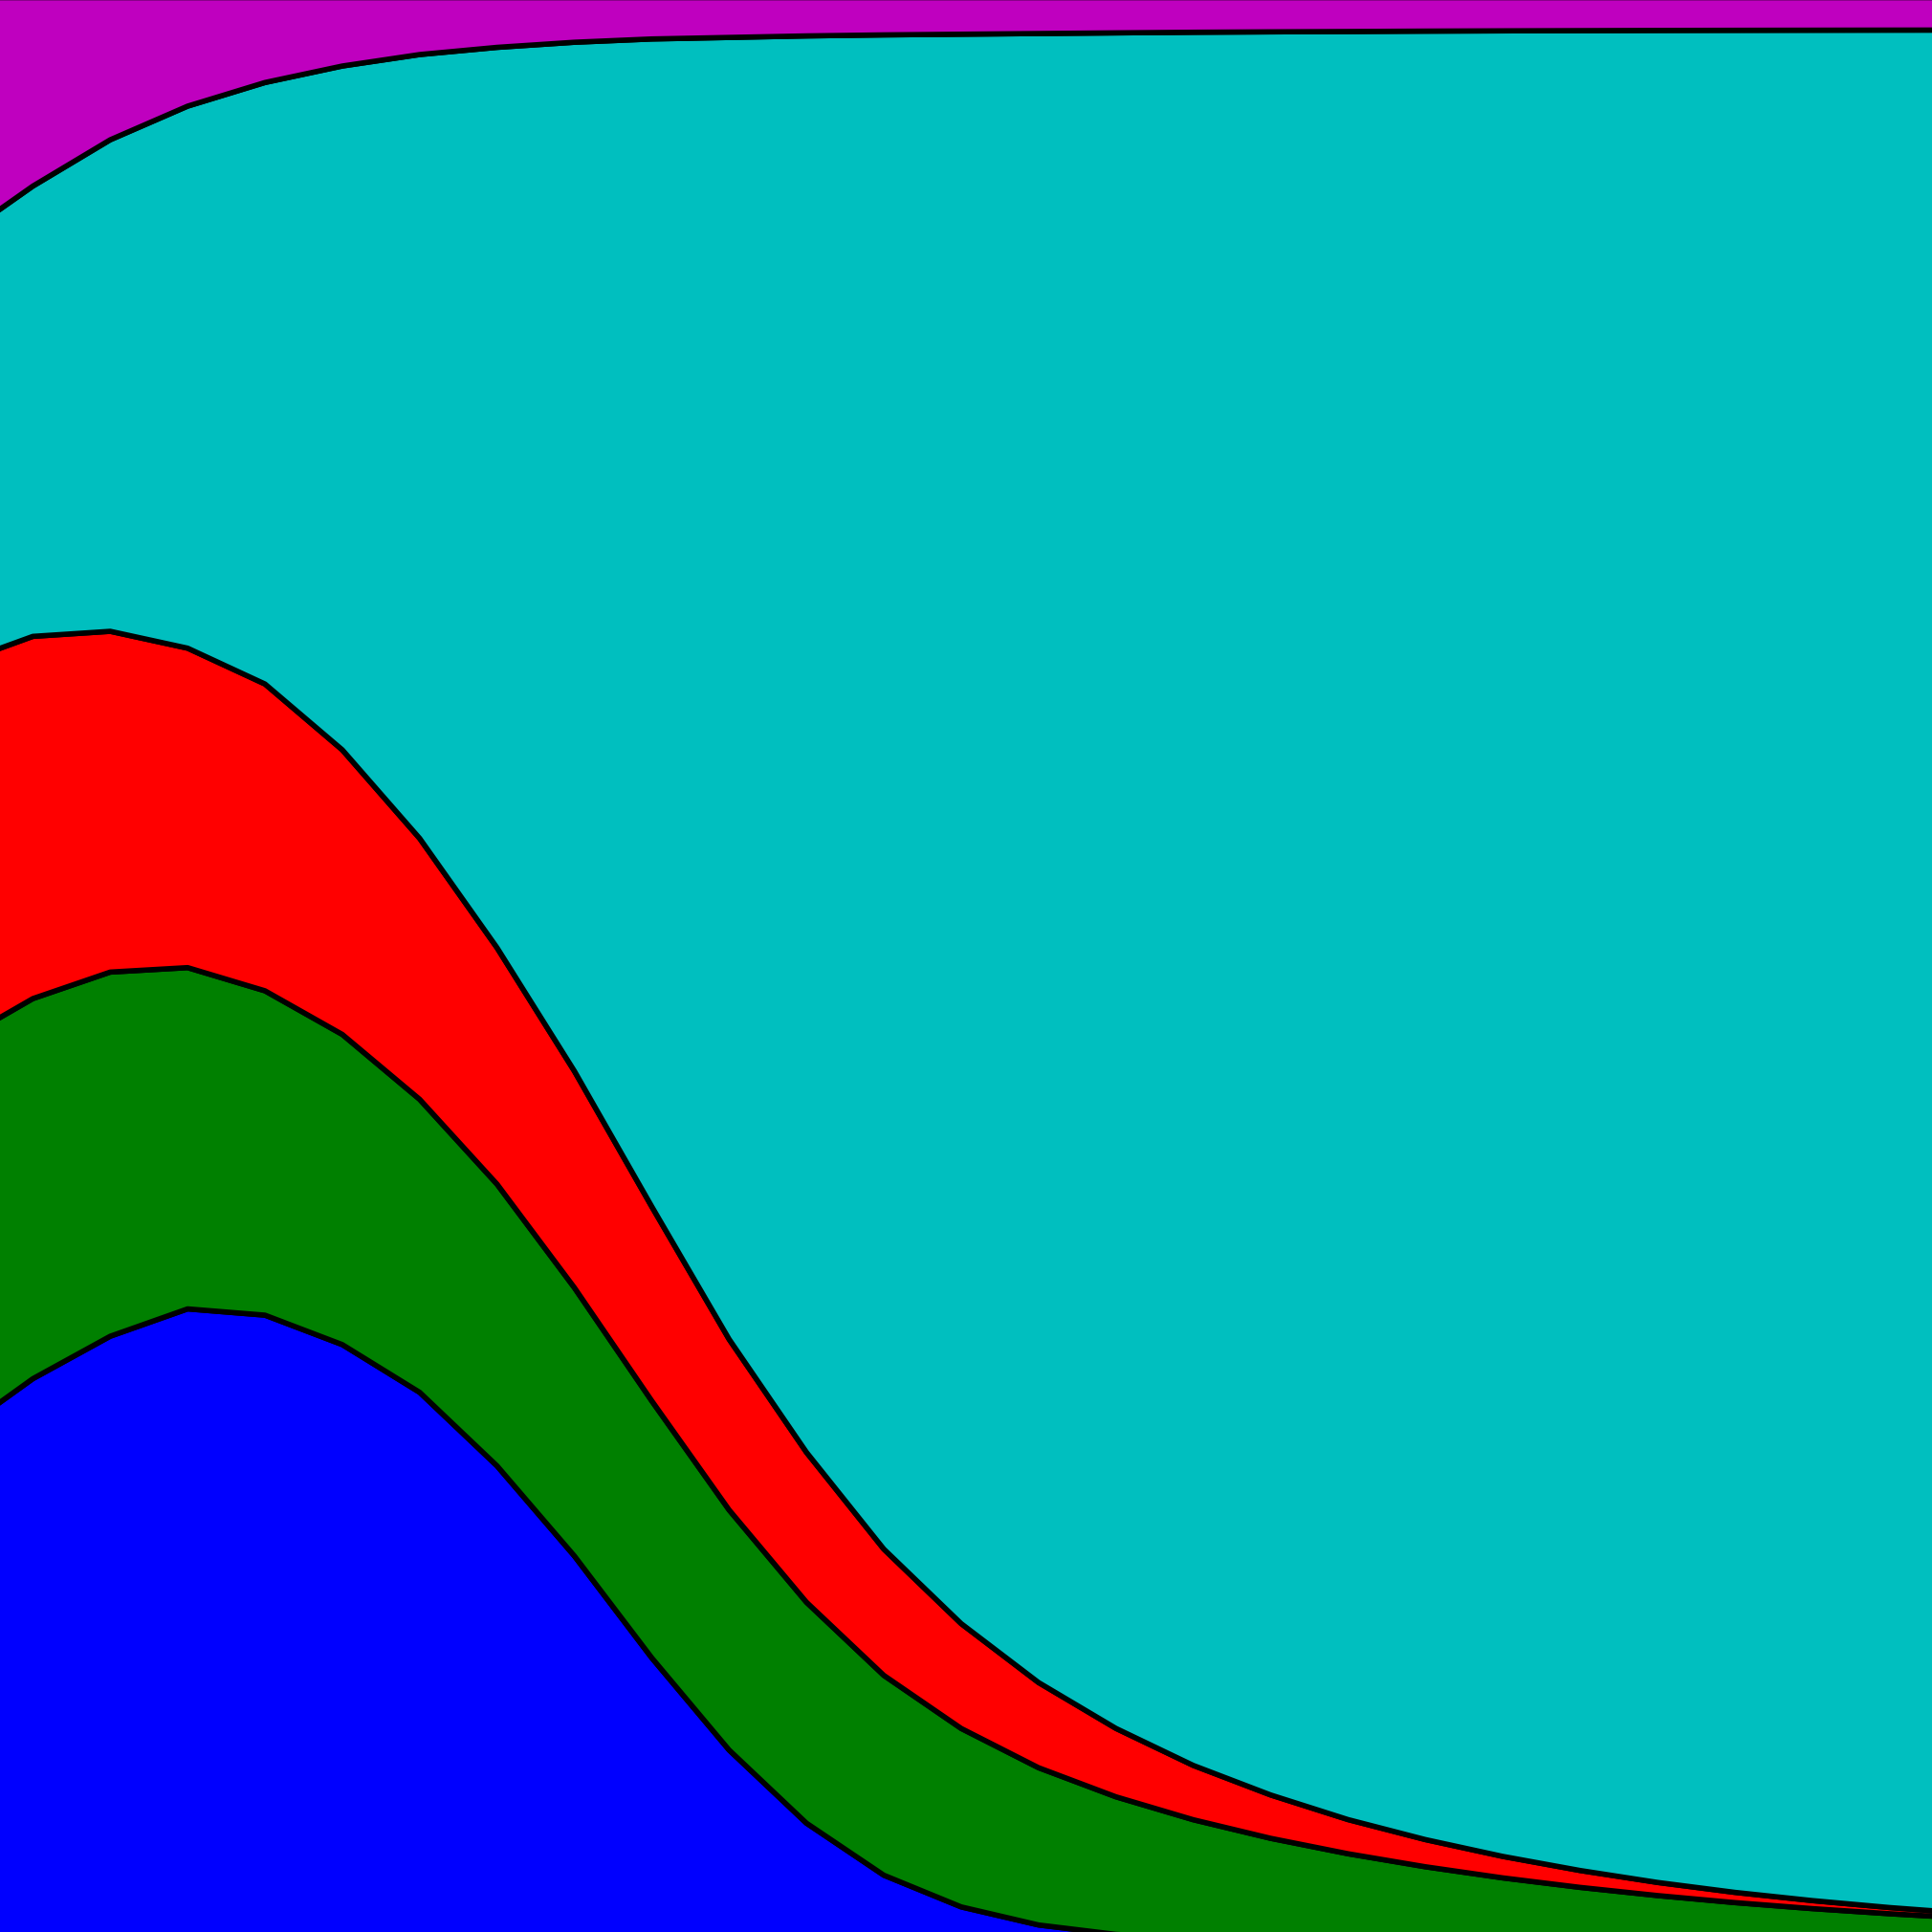
\includegraphics[height=3cm]{\assetsfolder/axelrod_logo.png}
                       \end{center}
                   \end{column}
               \end{columns}
        \end{center}

    \end{frame}

    \begin{frame}
        \documentclass[tikz]{standalone}

\usepackage{tikz}

\begin{document}

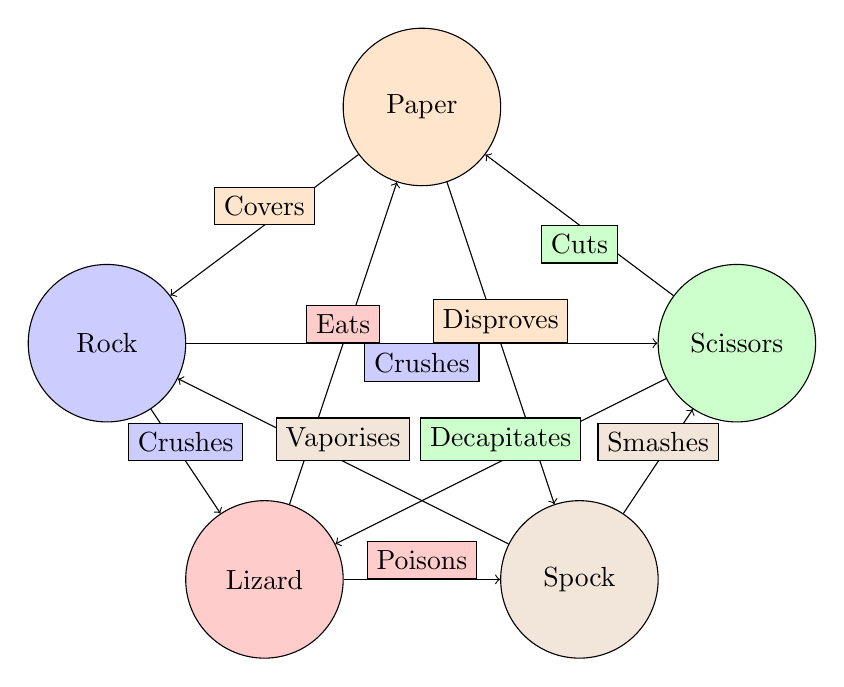
\begin{tikzpicture}

\node (R) at (0,0) [circle, minimum width = 2cm, draw, fill=blue!20] {Rock};
\node (P) at (4,3) [circle, minimum width = 2cm, draw, fill=orange!20] {Paper};
\node (S) at (8,0) [circle, minimum width = 2cm, draw, fill=green!20] {Scissors};
\node (Lz) at (2,-3) [circle, minimum width = 2cm, draw, fill=red!20] {Lizard};
\node (Sp) at (6,-3) [circle, minimum width = 2cm, draw, fill=brown!20] {Spock};

\draw [->] (P) -- node[above, fill=orange!20, draw] {Covers} (R);
\draw [->] (P) -- node[above, fill=orange!20, draw] {Disproves} (Sp);

\draw [->] (R) -- node[below, fill=blue!20, draw] {Crushes} (S);
\draw [->] (R) -- node[above, fill=blue!20, draw] {Crushes} (Lz);

\draw [->] (S) -- node[below, fill=green!20, draw] {Cuts} (P);
\draw [->] (S) -- node[above, fill=green!20, draw] {Decapitates} (Lz);

\draw [->] (Lz) -- node[above, fill=red!20, draw] {Eats} (P);
\draw [->] (Lz) -- node[above, fill=red!20, draw] {Poisons} (Sp);

\draw [->] (Sp) -- node[above, fill=brown!20, draw] {Vaporises} (R);
\draw [->] (Sp) -- node[above, fill=brown!20, draw] {Smashes} (S);
\end{tikzpicture}
\end{document}

    \end{frame}

    \begin{frame}
        \begin{center}
            \begin{tcolorbox}[colback=twitter,colframe=twitter!40!black,title=
                    \href{https://twitter.com/kirstyjean/status/870415613746962432}
                    {@kirstyjean} (2 Jun 2017):
]
                    Me: sets up flawless heat competition trial, lizards will
                    fight over hot podium, there can only be one winner!

                    Lizards:

                    \#ALlizards2017
           \end{tcolorbox}
        \end{center}
            %\end{column}
        %\end{columns}
        \begin{center}
            \pause
            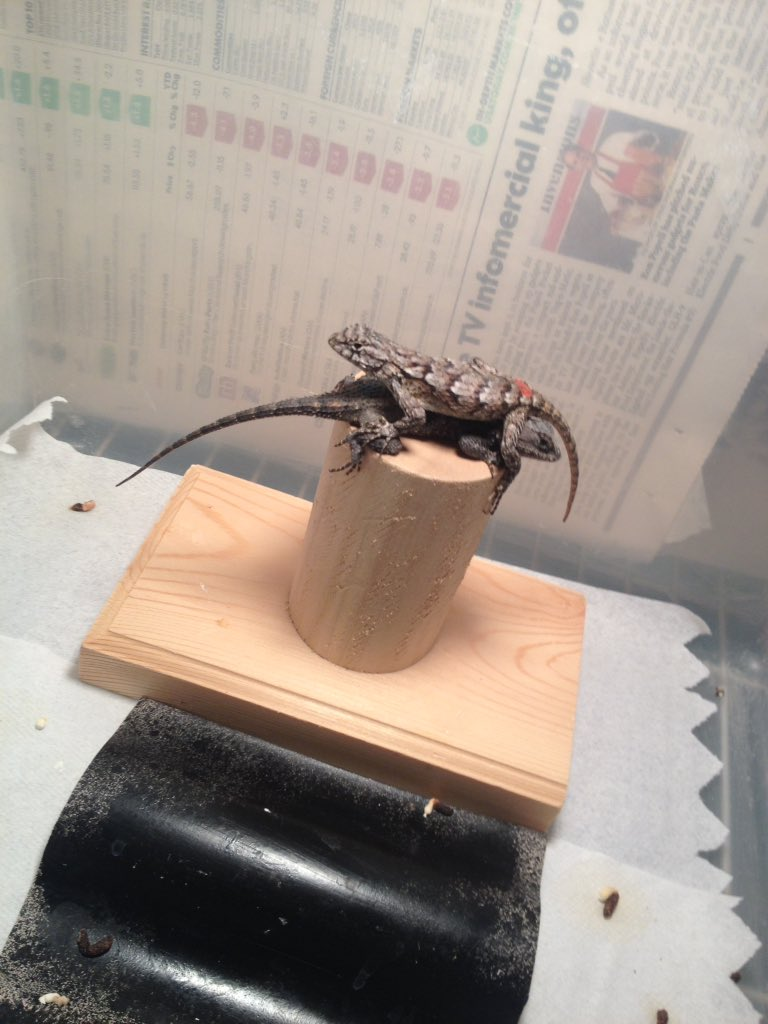
\includegraphics[width=.4\textwidth]
            {\assetsfolder/lizard-cooperation.jpg}
        \end{center}

    \end{frame}
    %\begin{frame}[fragile]{}
        %\begin{center}
            %\begin{minipage}{0.7\textwidth}
                %\begin{minted}[linenos, fontsize=\ssmall]{python}
%def moran(N, game, i=1, seed=0):
    %"""
    %Return the population counts for the Moran process on a game
    %"""
    %population = [0 for _ in range(i)] + [1 for _ in range(N - i)]
    %counts = [(i, N - i)]

    %np.random.seed(seed)

    %while len(set(population)) == 2:

        %scores = []

        %for i, player in enumerate(population):
            %total = 0
            %for j, opponent in enumerate(population):
                %if i != j:
                    %total += game[player, opponent]
            %scores.append(total)

        %total_score = sum(scores)
        %probabilities = [score / total_score for score in scores]
        %reproduce_index = np.random.choice(range(N), p=probabilities)

        %eliminate_index = np.random.randint(N)
        %population[eliminate_index] = population[reproduce_index]

        %counts.append((population.count(0), population.count(1)))
    %return counts
            %\end{minted}
        %\end{minipage}
    %\end{center}
%\end{frame}

    %\begin{frame}[fragile]{}
        %\begin{center}
            %\begin{minipage}{0.7\textwidth}
                %\begin{minted}[linenos, fontsize=\scriptsize, firstnumber=14]{python}
    %for i, player in enumerate(population):
        %total = 0
        %for j, opponent in enumerate(population):
            %if i != j:
                %total += game[player, opponent]
        %scores.append(total)

    %total_score = sum(scores)
    %probabilities = [score / total_score for score in scores]
    %reproduce_index = np.random.choice(range(N), p=probabilities)

    %eliminate_index = np.random.randint(N)
    %population[eliminate_index] = population[reproduce_index]
            %\end{minted}
        %\end{minipage}
    %\end{center}
%\end{frame}

    \begin{frame}
        \begin{center}
            \url{https://www.youtube.com/watch?v=p3Uos2fzIJ0}
        \end{center}
    \end{frame}

    \begin{frame}
        % PD
        \Huge
        \[
            \begin{pmatrix}
                3 & 0\\
                5 & 1
            \end{pmatrix}
            \qquad
            \begin{pmatrix}
                3 & 5\\
                0 & 1
            \end{pmatrix}
        \]

        \pause
		\normalsize
        \begin{center}
            (3 teams of 2.)
        \end{center}
    \end{frame}

    \begin{frame}[fragile]{}
        \begin{columns}
            \begin{column}{.4\textwidth}
                \begin{center}
                    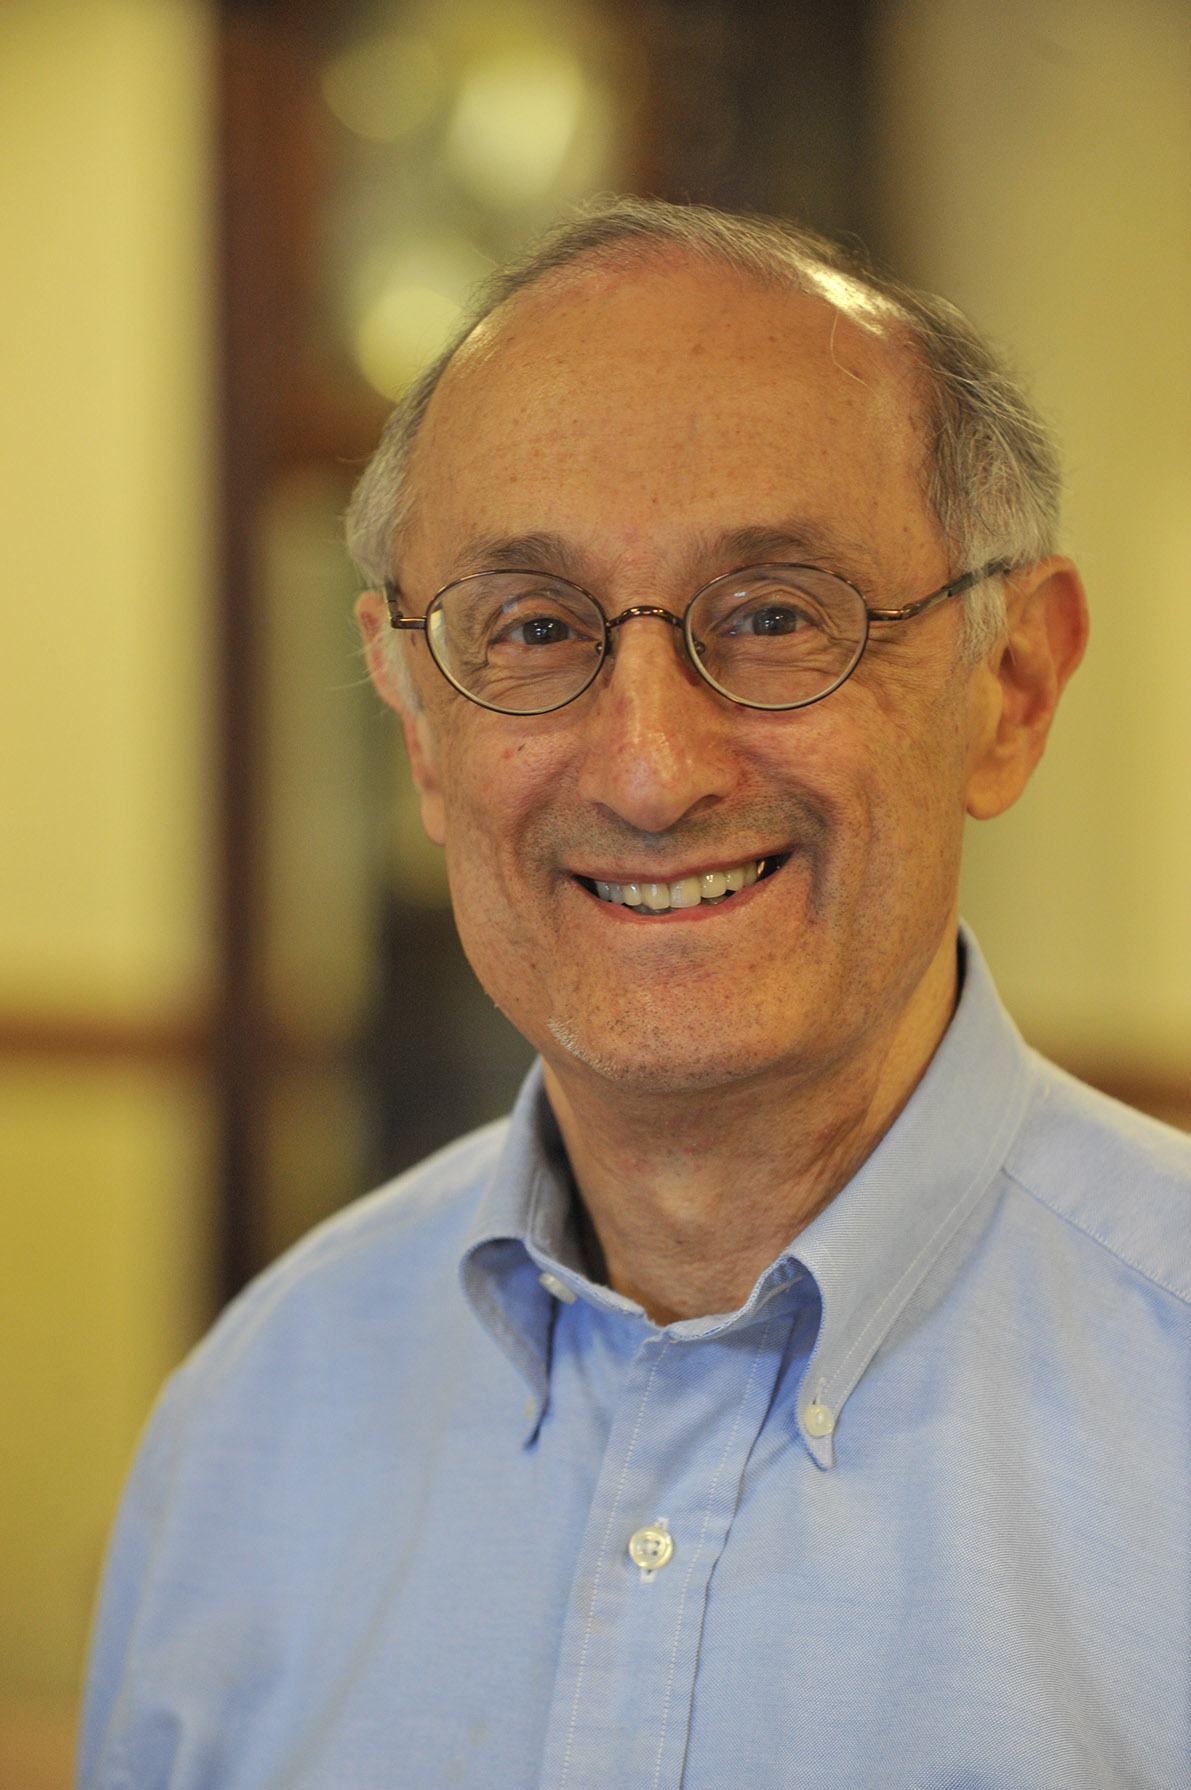
\includegraphics[width=.8\textwidth]{\assetsfolder/Axelrod.jpg}
                    \\
                    Robert Axelrod
                \end{center}
            \end{column}
            \pause
            \begin{column}{.6\textwidth}
                \begin{minted}[fontsize=\scriptsize]{python}
>>> import axelrod as axl

>>> players = (axl.TitForTat(),
...            axl.Cooperator())
>>> axl.Match(players, turns=5).play()
[(C, C), (C, C), (C, C), (C, C), (C, C)]

>>> players = (axl.TitForTat(),
...            axl.Defector())
>>> axl.Match(players, turns=5).play()
[(C, D), (D, D), (D, D), (D, D), (D, D)]

>>> players = (axl.TitForTat(),
...            axl.Alternator())
>>> axl.Match(players, turns=5).play()
[(C, C), (C, D), (D, C), (C, D), (D, C)]

                \end{minted}
            \end{column}
        \end{columns}
\end{frame}


    \begin{frame}
        \begin{center}
            \scalebox{.6}{\documentclass{standalone}
\usepackage{tikz}
\usetikzlibrary{calc, shapes, patterns}

\begin{document}
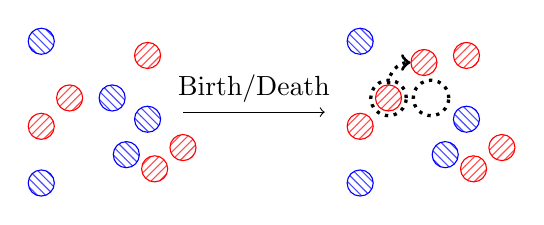
\begin{tikzpicture}[scale=.9]
	\node (A1) at (-1, -1) [circle, pattern=north west lines, pattern
        color=blue!70, draw=blue] {};
	\node (A2) at (-1, 1) [circle, pattern=north west lines, pattern
        color=blue!70, draw=blue] {};
	\node (A3) at (0, .2) [circle, pattern=north west lines, pattern
        color=blue!70, draw=blue] {};
	\node (A4) at (.2, -.6) [circle, pattern=north west lines, pattern
        color=blue!70, draw=blue] {};
	\node (A5) at (.5, -0.1) [circle, pattern=north west lines, pattern
        color=blue!70, draw=blue] {};
	\node (B1) at (-1, -.2) [circle, pattern=north east lines, pattern
        color=red!70, draw=red] {};
	\node (B2) at (1, -.5) [circle, pattern=north east lines, pattern
        color=red!70, draw=red] {};
	\node (B3) at (.5, .8) [circle, pattern=north east lines, pattern
        color=red!70, draw=red] {};
	\node (B4) at (-.6, .2) [circle, pattern=north east lines, pattern
        color=red!70, draw=red] {};
	\node (B5) at (.6, -.8) [circle, pattern=north east lines, pattern
        color=red!70, draw=red] {};

	\draw [->] (1, 0) -- (3, 0) node [above, pos=0.5] {Birth/Death};

	\node (A1) at ($(A1) + (4.5, 0)$) [circle, pattern=north west lines,
        pattern color=blue!70, draw=blue] {};
	\node (A2) at ($(A2) + (4.5, 0)$) [circle, pattern=north west lines,
        pattern color=blue!70, draw=blue] {};
	\node (A3) at ($(A3) + (4.5, 0)$) {};
	\node (A4) at ($(A4) + (4.5, 0)$) [circle, pattern=north west lines,
        pattern color=blue!70, draw=blue] {};
    \node (A5) at ($(A5) + (4.5, 0)$) [circle, pattern=north west lines,
        pattern color=blue!70, draw=blue] {};
	\node (B1) at ($(B1) + (4.5, 0)$) [circle, pattern=north east lines,
        pattern color=red!70, draw=red] {};
	\node (B2) at ($(B2) + (4.5, 0)$) [circle, pattern=north east lines,
        pattern color=red!70, draw=red] {};
	\node (B3) at ($(B3) + (4.5, 0)$) [circle, pattern=north east lines,
        pattern color=red!70, draw=red] {};
	\node (B4) at ($(B4) + (4.5, 0)$) [circle, pattern=north east lines,
        pattern color=red!70, draw=red] {};
	\node (B5) at ($(B5) + (4.5, 0)$) [circle, pattern=north east lines,
        pattern color=red!70, draw=red] {};

	\draw [dotted, very thick] (B4) circle (.25cm);
	\node (B6) at ($(B4) + (0.5, 0.5)$) [circle, pattern=north east lines,
        pattern color=red!70, draw=red] {};
	\draw [->, dotted, very thick] (B4) [out=90, in=180] to (B6);

	\draw [dotted, very thick] (A3) circle (.25cm);
\end{tikzpicture}
\end{document}
}
            % TODO Possibly re draw.
        \end{center}

		\pause

		  \begin{align*}
			  p_{i, i-1}&=\frac{i(N - i)}{N^2}\\
			  p_{i, i+1}&=\frac{i(N - i)}{N^2}\\
			  p_{i, i}&=1 - p_{i, i-1} - p_{i, i+1}
		  \end{align*}

    \end{frame}

\begin{frame}

    \begin{center}
        \textbf{Resistance}
        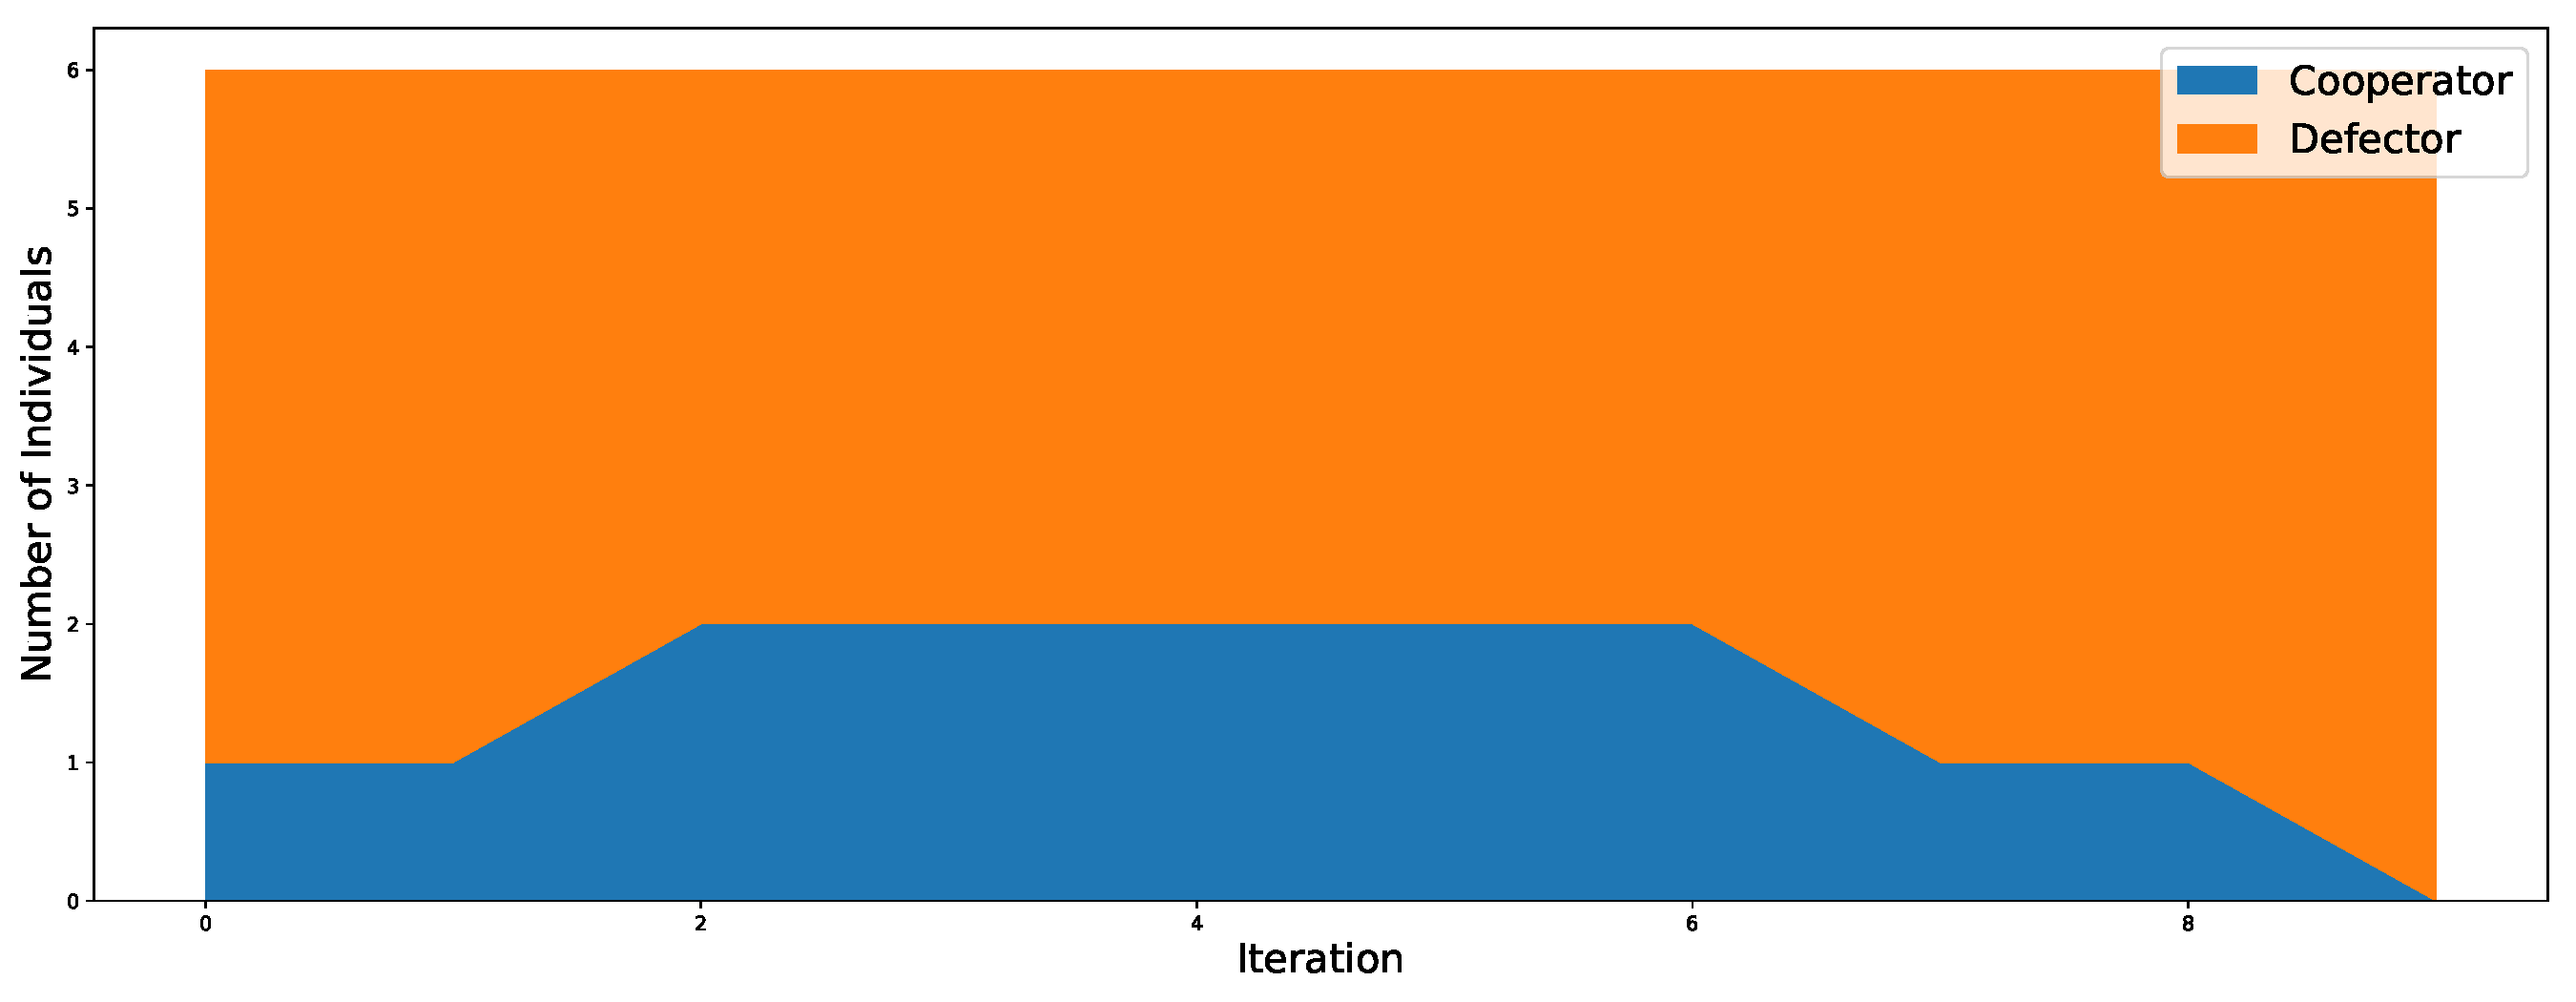
\includegraphics[height=.4\textheight]{\assetsfolder/moran_process_resistance.pdf}\\

        \textbf{Invasion}
        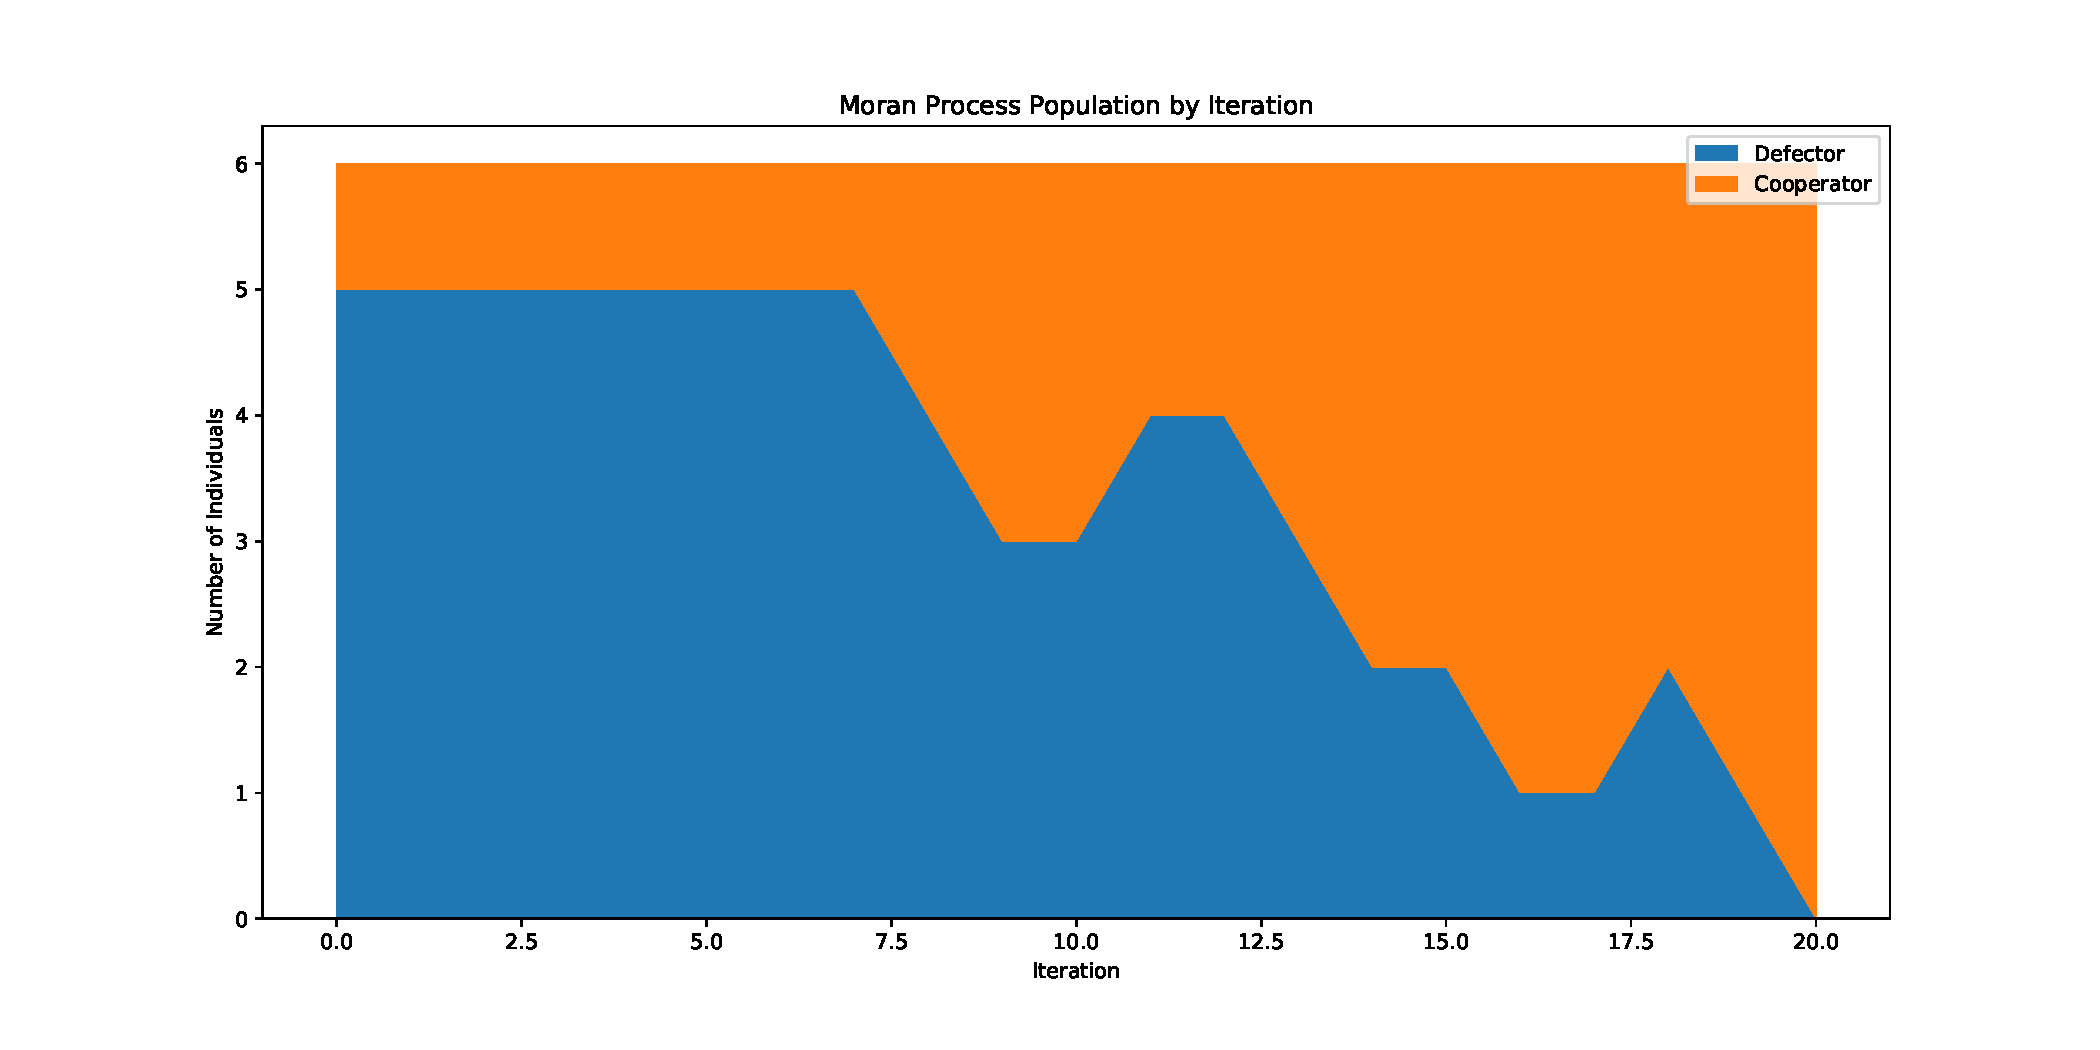
\includegraphics[height=.4\textheight]{\assetsfolder/moran_process_invasion.pdf}
    \end{center}
\end{frame}




\begin{frame}
    \scalebox{.7}{
        \input{\mlresearchfolder/assets/fsm.tex}
    }
\end{frame}

%\begin{frame}[fragile]{}

    %\begin{center}
        %\begin{minipage}{0.8\textwidth}
            %\begin{minted}[fontsize=\Huge]{python}
%import axelrod_dojo
            %\end{minted}
        %\end{minipage}
    %\end{center}
%\end{frame}


\begin{frame}
    \begin{center}
        \scalebox{.7}{
                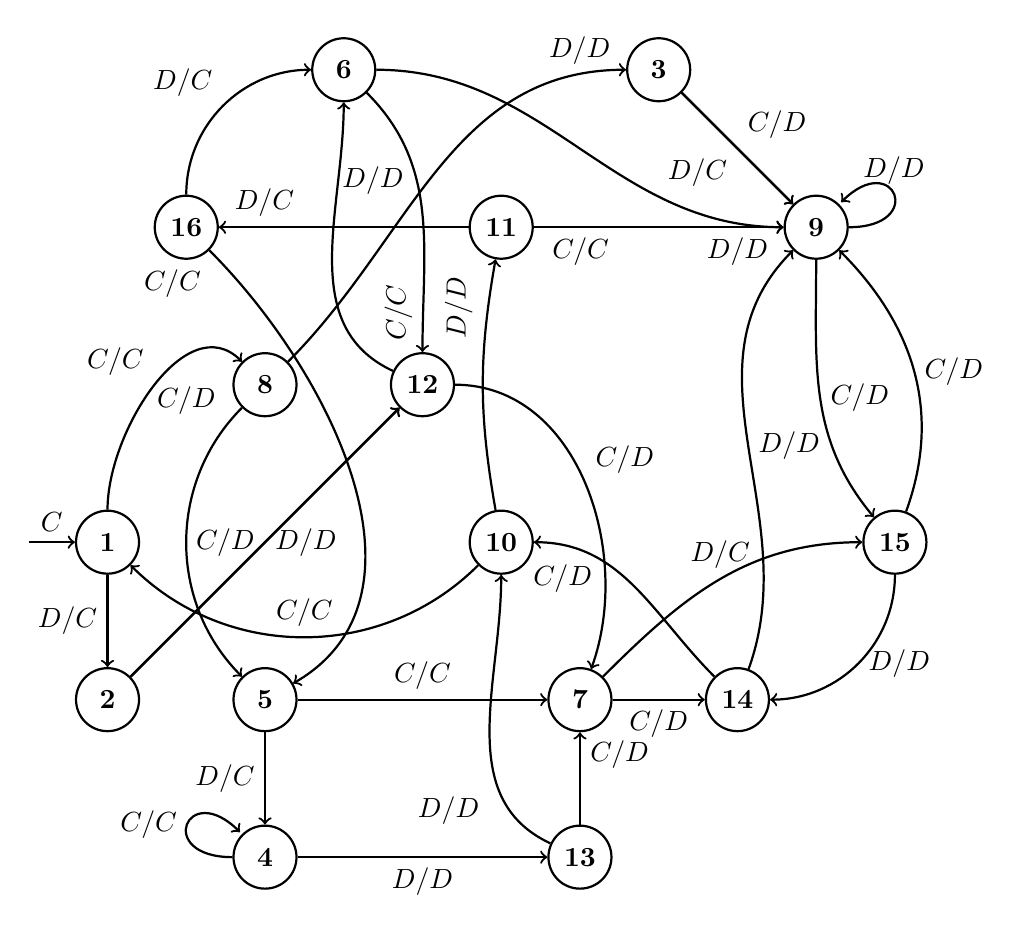
\begin{tikzpicture}

    \tikzstyle{state}=[minimum width=0.8cm, font=\boldmath];
    \node[circle, draw=black, thick] (5) at (0, 0) [state] {$6$};
	\node[circle, draw=black, thick] (2) at (4, 0) [state] {$3$};
	\node[circle, draw=black, thick] (15) at (-2, -2) [state] {$16$};
	\node[circle, draw=black, thick] (8) at ($(2)+(2,-2)$) [state] {$9$};
	\node[circle, draw=black, thick] (10) at ($(15)+(4, 0)$) [state] {$11$};
	
	\node[circle, draw=black, thick] (7) at ($(5)+(-1,-4)$) [state] {$8$};
	\node[circle, draw=black, thick] (11) at ($(7)+(2, 0)$) [state] {$12$};



	\node[circle, draw=black, thick] (9) at ($(10)+(0,-4)$) [state] {$10$};
	\node[circle, draw=black, thick] (0) at ($(9)+(-5,0)$) [state] {$1$};
	\node[circle, draw=black, thick] (14) at ($(9)+(5,0)$) [state] {$15$};

	\node[circle, draw=black, thick] (1) at ($(0)+(0,-2)$) [state] {$2$};
	\node[circle, draw=black, thick] (4) at ($(1)+(2,0)$) [state] {$5$};
	\node[circle, draw=black, thick] (6) at ($(4)+(4,0)$) [state] {$7$};
	\node[circle, draw=black, thick] (13) at ($(6)+(2,0)$) [state] {$14$};

	\node[circle, draw=black, thick] (3) at ($(4)+(0,-2)$) [state] {$4$};
	\node[circle, draw=black, thick] (12) at ($(6)+(0,-2)$) [state] {$13$};


    \coordinate[left of=0] (s);

    \draw (s) edge[out=0, in=180, ->, thick] node [above] {$C$} (0);
    \draw (0) edge[out=90, in=135, ->, thick] node [above left] {$C/C$} (7);
    \draw (0) edge[out=-90, in=90, ->, thick] node [left] {$D/C$} (1);

    \draw (1) edge[out=45, in=-135, ->, thick] node [left] {$C/D$} (11);
    \draw (1) edge[out=45, in=-135, ->, thick] node [right] {$D/D$} (11);
    
    \draw (2) edge[out=-45, in=135, ->, thick] node [above right] {$C/D$} (8);
    \draw (2) edge[out=-45, in=135, ->, thick] node [below left] {$D/C$} (8);

    \draw (3) edge[out=180, in=135, ->, thick, loop] node [left] {$C/C$} (3);
    \draw (3) edge[out=0, in=180, ->, thick] node [below] {$D/D$} (12);

    \draw (4) edge[out=0, in=180, ->, thick] node [above] {$C/C$} (6);
    \draw (4) edge[out=-90, in=90, ->, thick] node [left] {$D/C$} (3);

    \draw (5) edge[out=0, in=180, ->, thick] node [below, yshift=-1cm, xshift=2cm] {$D/D$} (8);
    \draw (5) edge[out=-45, in=90, ->, thick] node [left, yshift=-0.8cm, xshift=-0.3cm, rotate=90] {$C/C$} (11);

    \draw (6) edge[out=0, in=180, ->, thick] node [below] {$C/D$} (13);
    \draw (6) edge[out=45, in=180, ->, thick] node [above] {$D/C$} (14);

    \draw (7) edge[out=-135, in=135, ->, thick] node [yshift=1.8cm] {$C/D$} (4);
    \draw (7) edge[out=45, in=180, ->, thick] node [above, yshift=1.2cm, xshift=1.8cm] {$D/D$} (2);

    \draw (8) edge[out=0, in=45, ->, thick, loop] node [above] {$D/D$} (8);
    \draw (8) edge[out=-90, in=130, ->, thick] node [right] {$C/D$} (14);

    \draw (9) edge[out=-135, in=-45, ->, thick] node [above] {$C/C$} (0);
    \draw (9) edge[out=100, in=-100, ->, thick] node [above left, yshift=1.5cm, rotate=90] {$D/D$} (10);

    \draw (10) edge[out=0, in=180, ->, thick] node [below left, xshift=-0.5cm] {$C/C$} (8);
    \draw (10) edge[out=180, in=0, ->, thick] node [above left, xshift=-0.5cm] {$D/C$} (15);

    \draw (11) edge[out=0, in=70, ->, thick] node [above right] {$C/D$} (6);
    \draw (11) edge[out=155, in=-90, ->, thick] node [right, yshift=1cm] {$D/D$} (5);

    \draw (12) edge[out=90, in=-90, ->, thick] node [above right] {$C/D$} (6);
    \draw (12) edge[out=155, in=-90, ->, thick] node [left, yshift=-1cm] {$D/D$} (9);

    \draw (13) edge[out=135, in=0, ->, thick] node [below left, xshift=-0.4cm, yshift=0.4cm] {$C/D$} (9);
    \draw (13) edge[out=70, in=-135, ->, thick] node [right] {$D/D$} (8);

    \draw (14) edge[out=70, in=-45, ->, thick] node [right] {$C/D$} (8);
    \draw (14) edge[out=-90, in=0, ->, thick] node [right] {$D/D$} (13);

    \draw (15) edge[out=-45, in=30, ->, thick] node [left, xshift=-1.8cm, yshift=2.5cm] {$C/C$} (4);
    \draw (15) edge[out=90, in=180, ->, thick] node [above left] {$D/C$} (5);

    \end{tikzpicture}

        }
    \end{center}
\end{frame}


\begin{frame}
    \begin{center}
        
\includegraphics[height=.8\textheight]{./assets/hunger-games-hand-gesture.eps}


        \tiny
        \vfill
        \flushright{Image made by \url{http://www.freepik.com} from
        \url{https://www.flaticon.com} is licensed by CC BY 3.0}
    \end{center}
\end{frame}


\begin{frame}
            \footnotesize
            \begin{center}
                \textbf{Invasion (\(N=14\))}\\

                \input{\researchfolder/tex/summary_top_14_invade.tex}
            \end{center}
\end{frame}
\begin{frame}
            \footnotesize
            \begin{center}
                \textbf{Resistance (\(N=14\))}\\

                \input{\researchfolder/tex/summary_top_14_resist.tex}
            \end{center}
\end{frame}


\begin{frame}
    \begin{center}
        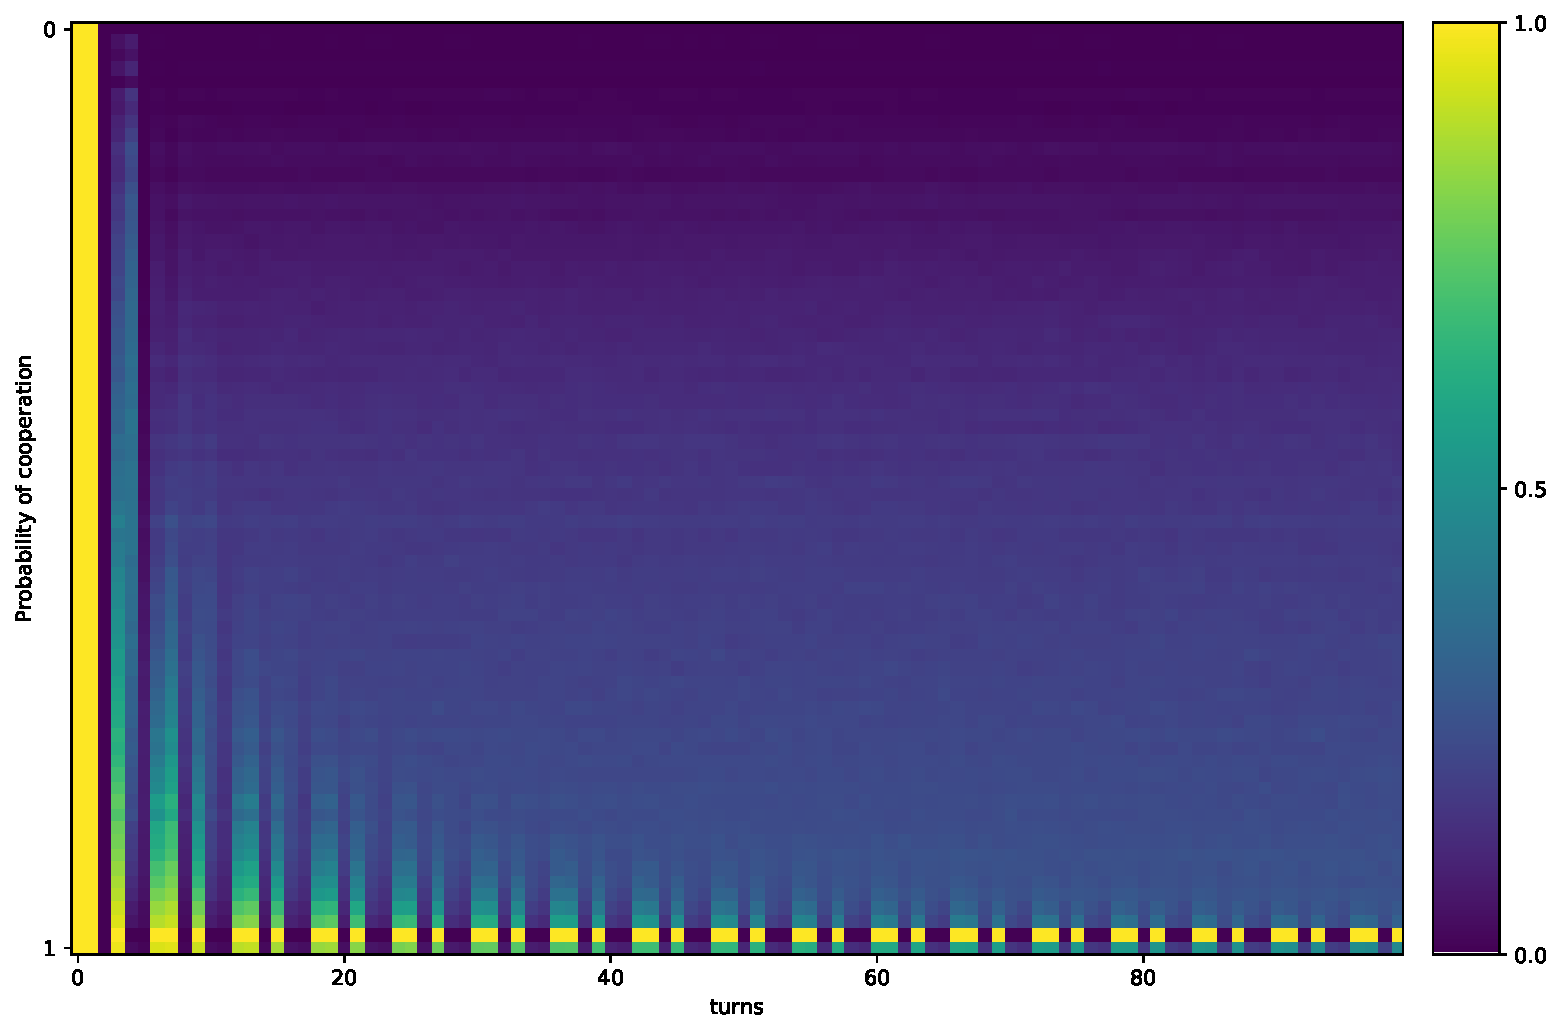
\includegraphics[width=.9\textwidth]{\assetsfolder/tf1_transitive_fingerprint.pdf}
    \end{center}
\end{frame}

\begin{frame}
    \begin{columns}
        \begin{column}{.6\textwidth}
            \begin{center}
                \scalebox{.49}{
                        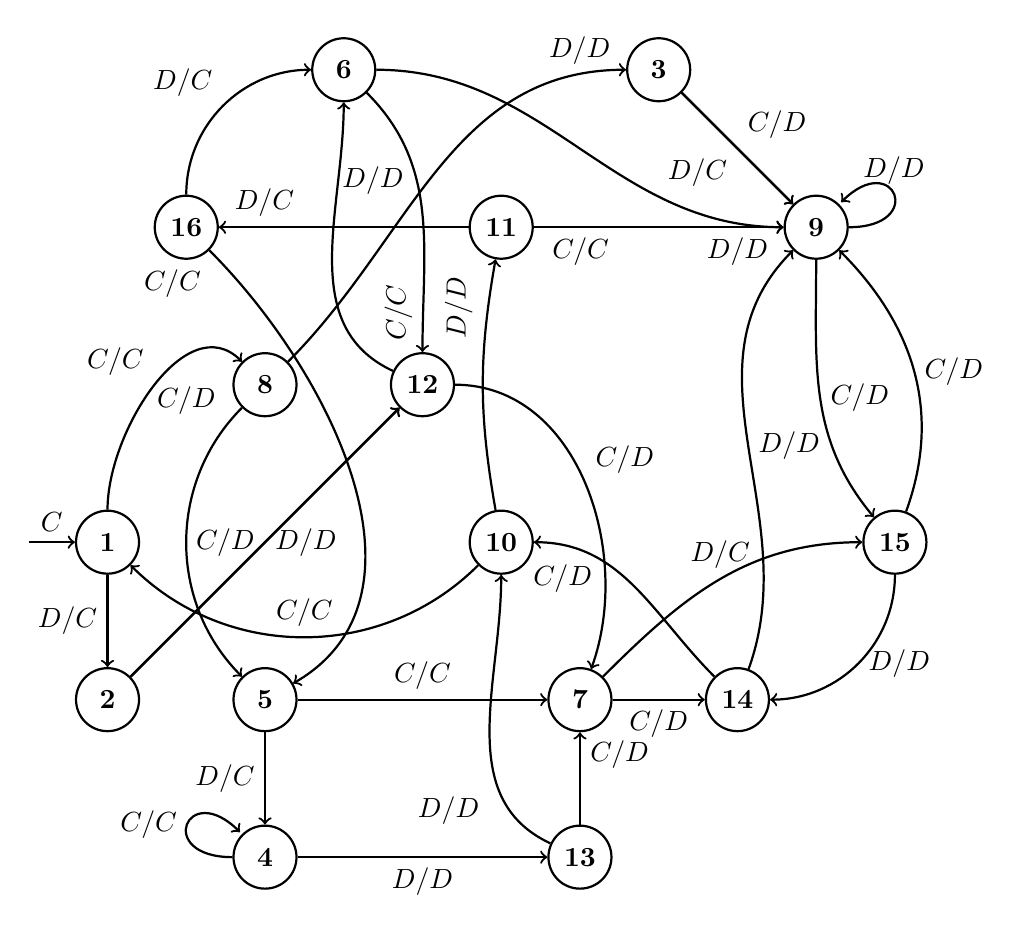
\begin{tikzpicture}

    \tikzstyle{state}=[minimum width=0.8cm, font=\boldmath];
    \node[circle, draw=black, thick] (5) at (0, 0) [state] {$6$};
	\node[circle, draw=black, thick] (2) at (4, 0) [state] {$3$};
	\node[circle, draw=black, thick] (15) at (-2, -2) [state] {$16$};
	\node[circle, draw=black, thick] (8) at ($(2)+(2,-2)$) [state] {$9$};
	\node[circle, draw=black, thick] (10) at ($(15)+(4, 0)$) [state] {$11$};
	
	\node[circle, draw=black, thick] (7) at ($(5)+(-1,-4)$) [state] {$8$};
	\node[circle, draw=black, thick] (11) at ($(7)+(2, 0)$) [state] {$12$};



	\node[circle, draw=black, thick] (9) at ($(10)+(0,-4)$) [state] {$10$};
	\node[circle, draw=black, thick] (0) at ($(9)+(-5,0)$) [state] {$1$};
	\node[circle, draw=black, thick] (14) at ($(9)+(5,0)$) [state] {$15$};

	\node[circle, draw=black, thick] (1) at ($(0)+(0,-2)$) [state] {$2$};
	\node[circle, draw=black, thick] (4) at ($(1)+(2,0)$) [state] {$5$};
	\node[circle, draw=black, thick] (6) at ($(4)+(4,0)$) [state] {$7$};
	\node[circle, draw=black, thick] (13) at ($(6)+(2,0)$) [state] {$14$};

	\node[circle, draw=black, thick] (3) at ($(4)+(0,-2)$) [state] {$4$};
	\node[circle, draw=black, thick] (12) at ($(6)+(0,-2)$) [state] {$13$};


    \coordinate[left of=0] (s);

    \draw (s) edge[out=0, in=180, ->, thick] node [above] {$C$} (0);
    \draw (0) edge[out=90, in=135, ->, thick] node [above left] {$C/C$} (7);
    \draw (0) edge[out=-90, in=90, ->, thick] node [left] {$D/C$} (1);

    \draw (1) edge[out=45, in=-135, ->, thick] node [left] {$C/D$} (11);
    \draw (1) edge[out=45, in=-135, ->, thick] node [right] {$D/D$} (11);
    
    \draw (2) edge[out=-45, in=135, ->, thick] node [above right] {$C/D$} (8);
    \draw (2) edge[out=-45, in=135, ->, thick] node [below left] {$D/C$} (8);

    \draw (3) edge[out=180, in=135, ->, thick, loop] node [left] {$C/C$} (3);
    \draw (3) edge[out=0, in=180, ->, thick] node [below] {$D/D$} (12);

    \draw (4) edge[out=0, in=180, ->, thick] node [above] {$C/C$} (6);
    \draw (4) edge[out=-90, in=90, ->, thick] node [left] {$D/C$} (3);

    \draw (5) edge[out=0, in=180, ->, thick] node [below, yshift=-1cm, xshift=2cm] {$D/D$} (8);
    \draw (5) edge[out=-45, in=90, ->, thick] node [left, yshift=-0.8cm, xshift=-0.3cm, rotate=90] {$C/C$} (11);

    \draw (6) edge[out=0, in=180, ->, thick] node [below] {$C/D$} (13);
    \draw (6) edge[out=45, in=180, ->, thick] node [above] {$D/C$} (14);

    \draw (7) edge[out=-135, in=135, ->, thick] node [yshift=1.8cm] {$C/D$} (4);
    \draw (7) edge[out=45, in=180, ->, thick] node [above, yshift=1.2cm, xshift=1.8cm] {$D/D$} (2);

    \draw (8) edge[out=0, in=45, ->, thick, loop] node [above] {$D/D$} (8);
    \draw (8) edge[out=-90, in=130, ->, thick] node [right] {$C/D$} (14);

    \draw (9) edge[out=-135, in=-45, ->, thick] node [above] {$C/C$} (0);
    \draw (9) edge[out=100, in=-100, ->, thick] node [above left, yshift=1.5cm, rotate=90] {$D/D$} (10);

    \draw (10) edge[out=0, in=180, ->, thick] node [below left, xshift=-0.5cm] {$C/C$} (8);
    \draw (10) edge[out=180, in=0, ->, thick] node [above left, xshift=-0.5cm] {$D/C$} (15);

    \draw (11) edge[out=0, in=70, ->, thick] node [above right] {$C/D$} (6);
    \draw (11) edge[out=155, in=-90, ->, thick] node [right, yshift=1cm] {$D/D$} (5);

    \draw (12) edge[out=90, in=-90, ->, thick] node [above right] {$C/D$} (6);
    \draw (12) edge[out=155, in=-90, ->, thick] node [left, yshift=-1cm] {$D/D$} (9);

    \draw (13) edge[out=135, in=0, ->, thick] node [below left, xshift=-0.4cm, yshift=0.4cm] {$C/D$} (9);
    \draw (13) edge[out=70, in=-135, ->, thick] node [right] {$D/D$} (8);

    \draw (14) edge[out=70, in=-45, ->, thick] node [right] {$C/D$} (8);
    \draw (14) edge[out=-90, in=0, ->, thick] node [right] {$D/D$} (13);

    \draw (15) edge[out=-45, in=30, ->, thick] node [left, xshift=-1.8cm, yshift=2.5cm] {$C/C$} (4);
    \draw (15) edge[out=90, in=180, ->, thick] node [above left] {$D/C$} (5);

    \end{tikzpicture}

                }
            \end{center}
        \end{column}

        \begin{column}{.4\textwidth}
            \small
            \begin{tabular}{ll}
                \toprule
                TF1 \#1   & TF1 \#2\\
                \midrule
                \bf{1}: C & \bf{1}: C  \\
                \bf{8}: C & \bf{8}: C  \\
                \bf{5}: D & \bf{5}: D  \\
                4: C      & 4: C  \\
                4: C      & 4: C  \\
                4: C      & 4: C  \\
                4: C      & 4: C  \\
                4: C      & 4: C  \\
                \bottomrule
            \end{tabular}
        \end{column}
    \end{columns}
\end{frame}


\begin{frame}
    \Huge
    \begin{center}
        \only<1>{
            164
            }
        \only<2>{
            \sout{164}\; 211+
            }
    \end{center}
\end{frame}


\begin{frame}
    \begin{footnotesize}
        \begin{tcolorbox}[colback=github,colframe=blue!40!black,title=
                Julie Rymer - \href{https://gitter.im/Axelrod-Python/Axelrod?at=591388592b926f8a6741435d}
                {@Chadys} - (10 May 2017):
    ]
                And I really wanted to thank you all, I discovered your project because of a
                course where we needed to participate in an open source project, and I had the
                occasion to compare the welcome me and my coworkers received here compared to
                other people from my class who worked on different project. And I've got to said
                you are awesome on that part and on the help your provide to newbies  I like
                your project so I'll try to continue to contribute now and then !
       \end{tcolorbox}
    \end{footnotesize}

 \end{frame}

 \begin{frame}
    \begin{center}
        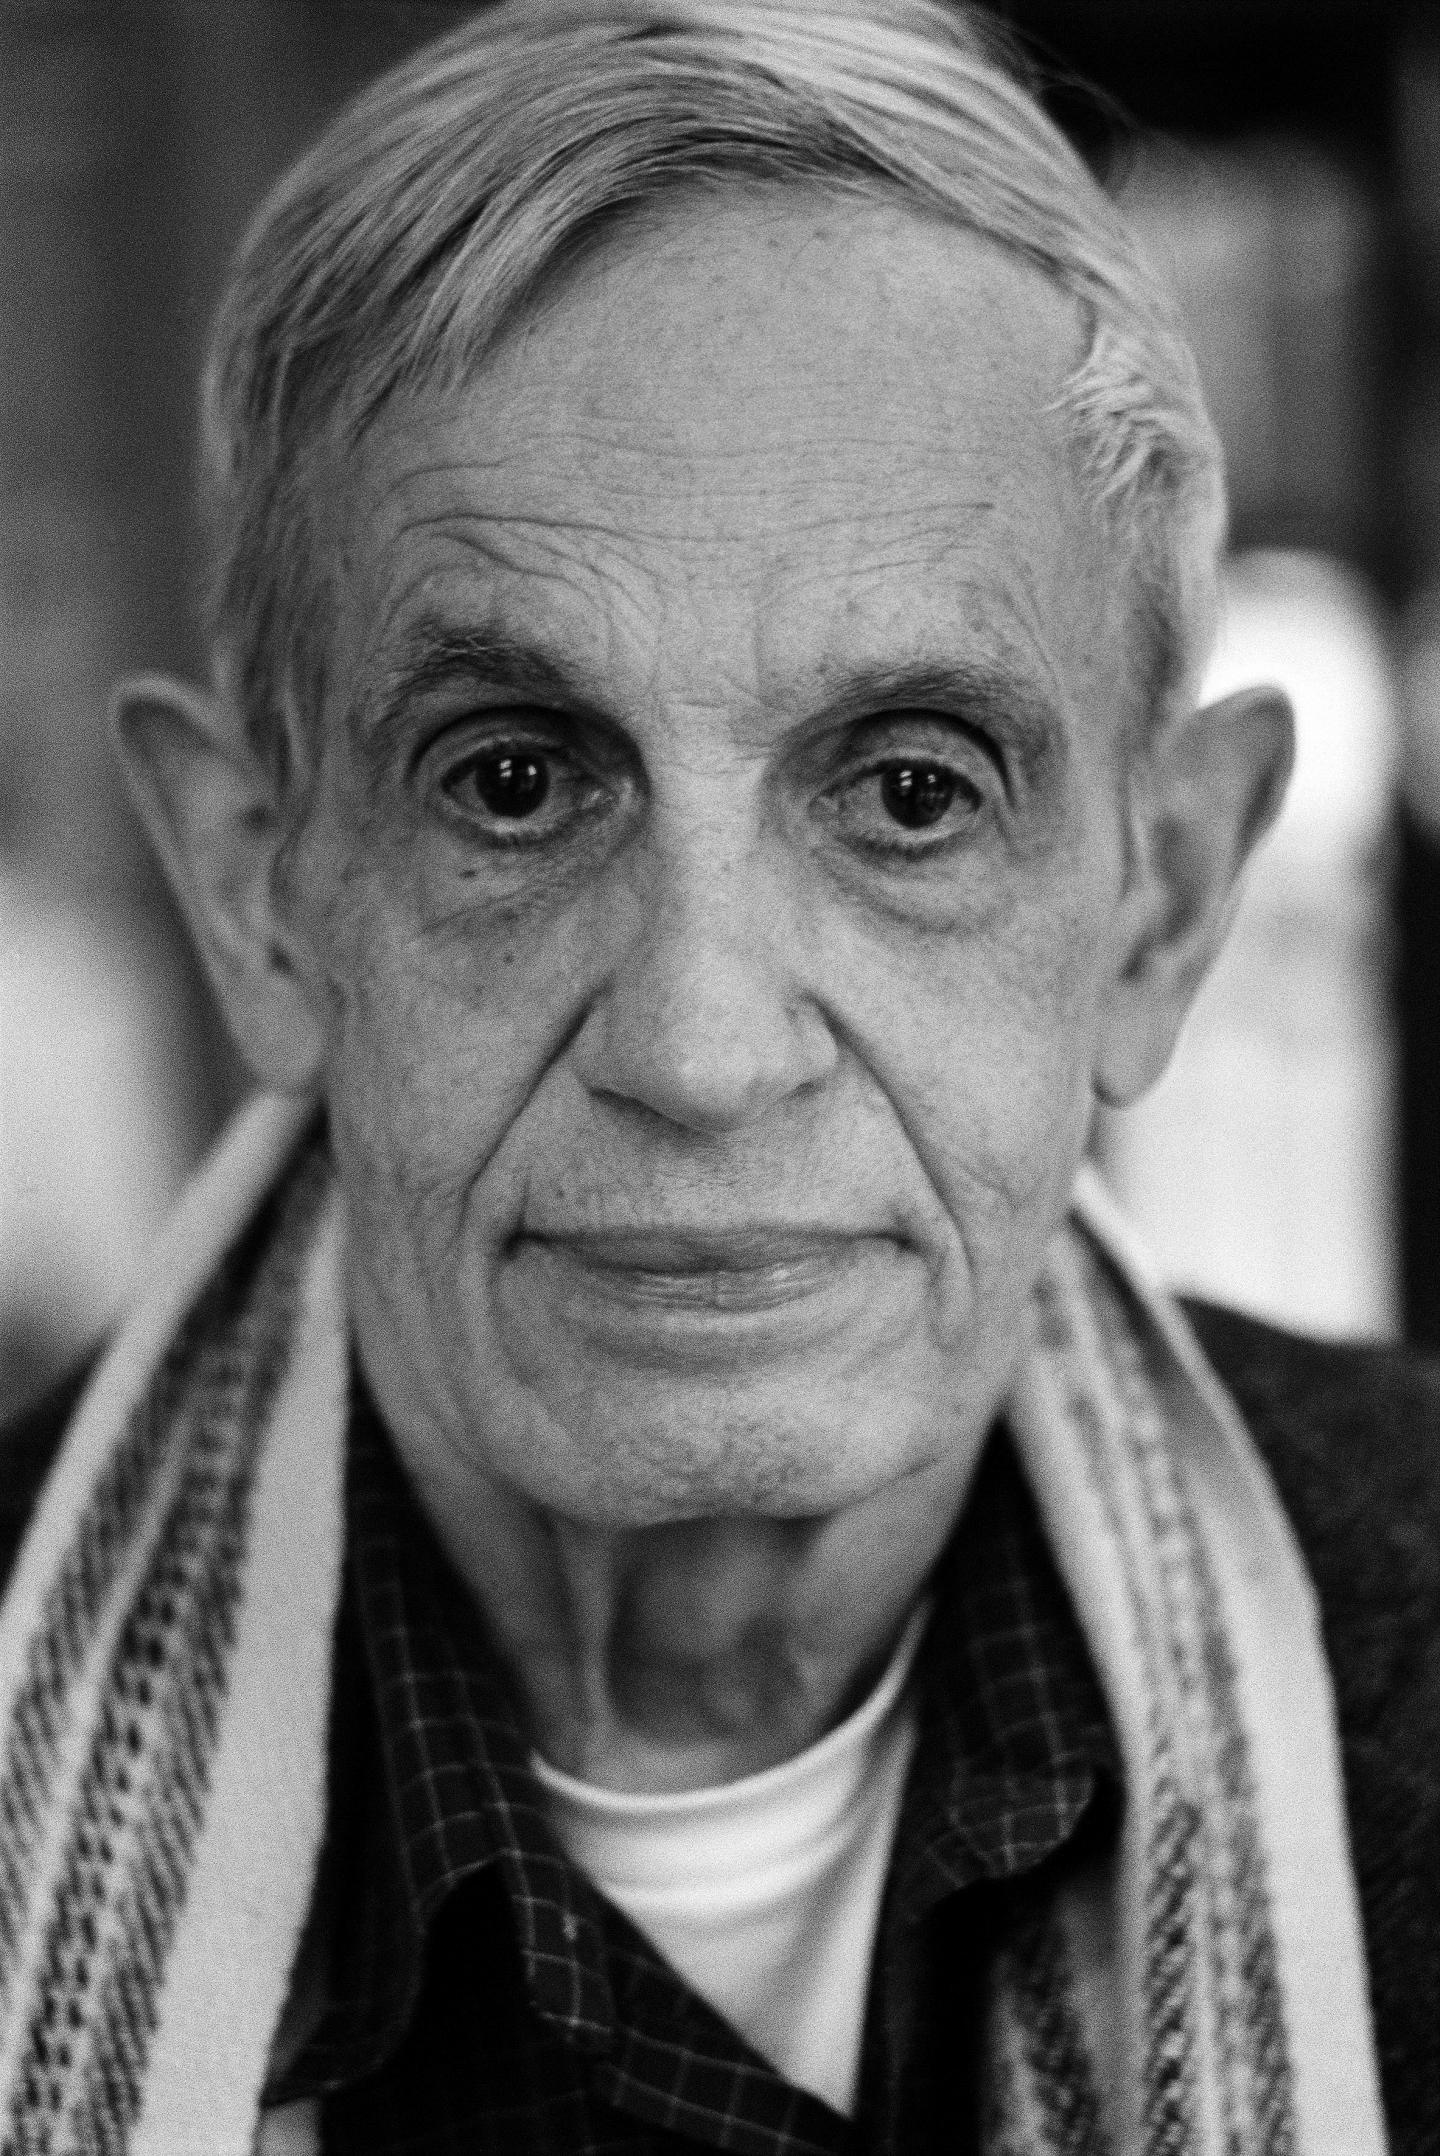
\includegraphics[height=.8\textheight]{\assetsfolder/nash.jpg}
        \\
        John Nash
    \end{center}
 \end{frame}

 \begin{frame}
    \begin{center}
        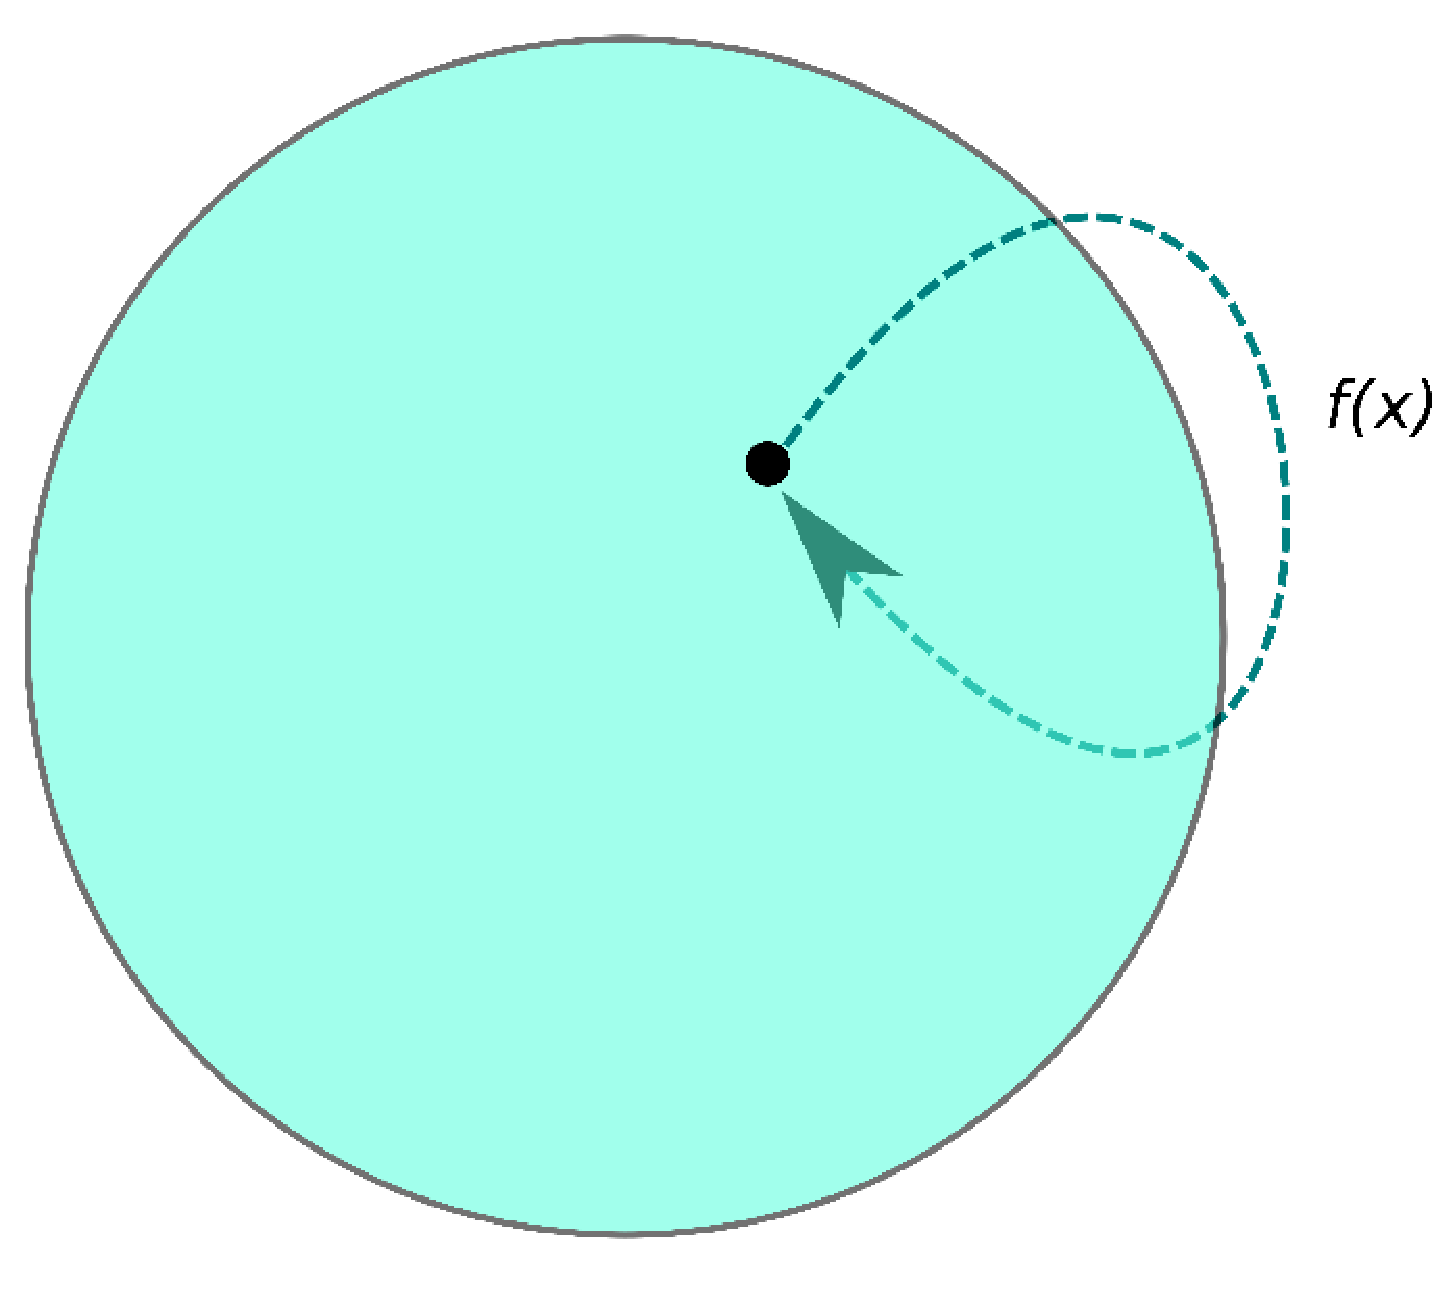
\includegraphics[height=.8\textheight]{\assetsfolder/brouwer_fixed_point_theorem.pdf}
    \end{center}
 \end{frame}

 \begin{frame}
   \begin{columns}
        \begin{column}{.35\textwidth}
            \begin{itemize}
                \item \href{https://twitter.com/NikoletaGlyn}{@NikoletaGlyn}
                \item \href{https://twitter.com/opcampbell}{@opcampbell}
                \item \href{http://marcharper.codes/}{marcharper.codes}
            \end{itemize}
        \end{column}
        \begin{column}{.65\textwidth}
            \begin{itemize}
                \item \href{https://github.com/Axelrod-Python/Axelrod}{github.com/Axelrod-Python/Axelrod}
                \item \href{https://gitter.im/Axelrod-Python/Axelrod}{gitter.im/Axelrod-Python/Axelrod}
                \item
                    \href{https://arxiv.org/abs/1707.06920}{arxiv.org/abs/1707.06920}
            \end{itemize}
        \end{column}
   \end{columns}

        \begin{center}
               \href{https://twitter.com/drvinceknight}{@drvinceknight}
        \end{center}

   \begin{columns}
        \begin{column}{.4\textwidth}
            \begin{itemize}
                \item
                    \href{https://vknight.org/gt/}{vknight.org/gt/}
            \end{itemize}
        \end{column}
        \begin{column}{.6\textwidth}
            \begin{itemize}
                \item \href{https://github.com/drvinceknight/Nashpy}{github.com/drvinceknight/Nashpy}
            \end{itemize}
        \end{column}
   \end{columns}
\end{frame}

\end{document}
